\documentclass[conference]{IEEEtran}

\usepackage{amsmath}
\usepackage{graphicx}
\usepackage{booktabs}
\usepackage{cite}
\usepackage{url}

\title{A Comparative Study of Machine Learning, Deep Learning, and Foundation Models for Short-Term Electricity Load Forecasting}

\author{
\IEEEauthorblockN{Author One}
\IEEEauthorblockA{\textit{Affiliation One}\\
City, Country\\
email1@example.com}
\and
\IEEEauthorblockN{Author Two}
\IEEEauthorblockA{\textit{Affiliation Two}\\
City, Country\\
email2@example.com}
}

\begin{document}
\maketitle

\begin{abstract}
Short-term electricity load forecasting is a core component of smart-grid operation, predictive planning, and industrial energy management. This paper presents a reproducible benchmark comparing two classical baselines (SeasonalNaive and a grid-tuned SARIMA), a tree model (XGBoost), three neural architectures (DLinear, PatchTST, iTransformer), and two time-series foundation models (Chronos-Bolt-Small and TimesFM~2.5). The primary evaluation uses the ECL electricity consumption dataset with aggregate load as the target. ETTh1 is used as a secondary industrial benchmark with HUFL, a load-related transformer variable, as the target; the oil-temperature variable OT is deliberately not treated as load. Experiments cover horizons of 24, 96, and 168 hours using a fixed 336-hour context. On ECL the top three models---TimesFM, Chronos-Bolt, and XGBoost---are within roughly $0.1$--$0.4\%$ of one another across horizons, with TimesFM marginally best at H=24 and XGBoost marginally best at H=96 and H=168; the grid-tuned SARIMA closes most of the remaining gap without learned features. On ETTh1/HUFL, Chronos-Bolt is best at H=24, while DLinear is best at H=96 and H=168. These results show that foundation models are competitive zero-shot forecasters, but classical and supervised models remain strong when training data and feature engineering are available.
\end{abstract}

\begin{IEEEkeywords}
short-term load forecasting, time series, deep learning, foundation models, SARIMA, XGBoost, smart grid
\end{IEEEkeywords}

\section{Introduction}
Short-term load forecasting (STLF) supports dispatch planning, balancing, tariff-aware operation, maintenance planning, and anomaly-aware industrial energy management. In modern smart-grid and Industry 4.0 settings, forecasting models are expected not only to be accurate, but also to be reproducible, computationally affordable, and robust across operating regimes.

The methodological landscape is broad. Classical methods such as ARIMA-family models and seasonal naive baselines remain common references; machine-learning models such as gradient boosting are attractive because they incorporate lag and calendar features with modest engineering cost; and recent deep-learning and foundation models promise broader transfer across time-series domains. This creates a practical question: when do expensive architectures or zero-shot foundation models actually improve over strong inexpensive baselines?

This paper reports a reproducible execution of the benchmark on two public datasets. The contribution is pragmatic: (i) an end-to-end repository with data validation, leakage-aware scaling, metrics, timing, figures, and paper generation; (ii) real results for SeasonalNaive, a grid-tuned SARIMA, XGBoost, DLinear, PatchTST, iTransformer, Chronos-Bolt-Small, and TimesFM~2.5; (iii) Diebold--Mariano tests computed from per-window errors; and (iv) an accuracy--latency analysis that separates practical deployment cost from raw accuracy.

\section{Related Work}
Classical time-series forecasting methods, in particular ARIMA-family models, remain important because they establish interpretable and inexpensive references; automatic order selection by information criteria such as AICc has made them practical to deploy on individual series \cite{hyndman2008automatic}. Machine-learning approaches based on lagged targets, calendar variables, and gradient-boosted trees are widely used in load forecasting because they are fast to train and robust under tabular feature engineering \cite{chen2016xgboost}. Deep-learning models such as LSTM \cite{hochreiter1997lstm}, attention-based architectures \cite{vaswani2017attention}, Informer \cite{zhou2021informer}, DLinear \cite{zeng2023dlinear}, PatchTST \cite{nie2023patchtst}, iTransformer \cite{liu2024itransformer}, and TimesNet \cite{wu2023timesnet} have broadened the long-horizon forecasting toolbox.

Time-series foundation models such as TimesFM~\cite{das2024timesfm} and the Chronos family~\cite{ansari2024chronos} motivate a new evaluation axis: no-task-specific-training inference versus supervised training on the target dataset. We evaluate the distilled Chronos-Bolt-Small variant from that family. A fair comparison must state that public benchmarks may have appeared in pretraining corpora, so zero-shot performance on ECL or ETT should not be interpreted as guaranteed dataset-unseen generalization.

\section{Methodology}
Given a univariate context window $\mathbf{x}_{t-L+1:t}$, the task is to predict $\hat{\mathbf{y}}_{t+1:t+H}$ for horizons $H \in \{24,96,168\}$. The executed experiments use a fixed context length of $L=336$ hours, which includes daily and weekly seasonal information and permits use of lag-168 features.

The SeasonalNaive baseline repeats the most recent daily seasonal pattern. The SARIMA baseline uses a fixed-grid AICc selection on the training split: candidate orders span $(p,d,q)\in\{(1,1,1),(2,1,1),(1,1,2),(2,1,2)\}$ with seasonal orders $(P,D,Q)_{24}\in\{(1,1,1),(2,1,1),(1,1,2)\}$, and the lowest-AICc fit is reused on every test window via state filtering on the new context (no per-window re-fit). XGBoost is trained as a direct multi-output regressor using lag-1, lag-24, lag-168, rolling means over 24 and 168 hours, and cyclic calendar features. DLinear, PatchTST, and iTransformer are trained through NeuralForecast in the same target-only setting, with a short validation-only learning-rate sweep over $\{10^{-3},5\cdot10^{-4}\}$ and early stopping. Neural training and evaluation use NeuralForecast's rolling-origin cross-validation: although the train, validation, and test segments are concatenated to construct the rolling windows, each window is predicted using only past observations, so no future information leaks into training. Chronos-Bolt-Small and TimesFM~2.5 are evaluated in zero-shot mode without task-specific training. All preprocessing for trained models is fitted only on the training split, and metrics are computed after inverse-transforming predictions to the original target scale. Foundation models and SARIMA are evaluated directly on the original target scale.

Figure~\ref{fig:methodology} summarizes the execution pipeline.

\begin{figure}[t]
  \centering
  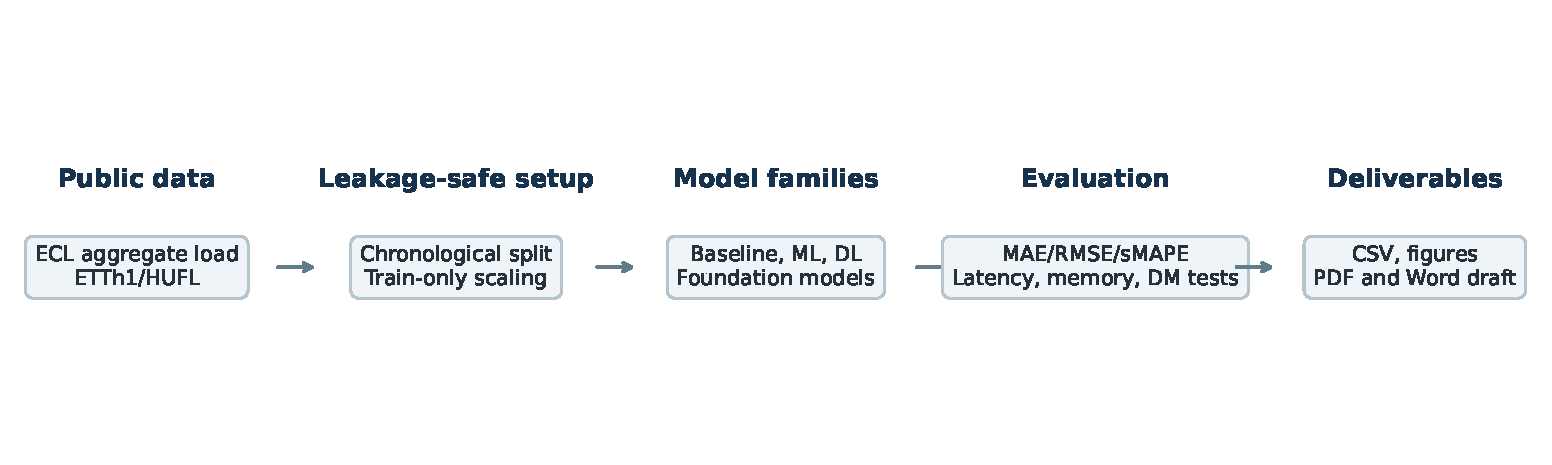
\includegraphics[width=\linewidth]{../figures/fig1_methodology.pdf}
  \caption{Experimental pipeline.}
  \label{fig:methodology}
\end{figure}

\section{Experimental Setup}
The primary dataset is ECL, processed as an aggregate hourly electricity load across 321 clients. The secondary dataset is ETTh1 with HUFL as the target. ETTh1 OT is oil temperature and is not used as electricity load. ECL is split chronologically into 70\% train, 10\% validation, and 20\% test. ETTh1 uses the standard 12-month, 4-month, 4-month chronological split.

Accuracy is measured with MAE, RMSE, sMAPE, and wMAPE. Efficiency is measured with training time, single-window inference latency (batch size~1), trainable parameters, and peak GPU memory. Trained models (XGBoost, DLinear, PatchTST, iTransformer) are evaluated across five seeds (42--46) and reported as mean~$\pm$~std; deterministic models (SeasonalNaive, SARIMA, Chronos-Bolt, TimesFM) are evaluated once and have a standard deviation of zero by construction. Diebold--Mariano tests are computed on per-window absolute errors for the top two models by MAE at seed 42 for each dataset and horizon. Because per-window averaging and flattened point-wise MAE weight errors differently, the statistical-test ranking can differ slightly from the table ranking when models are very close.

\section{Results}
\begin{figure}[t]
  \centering
  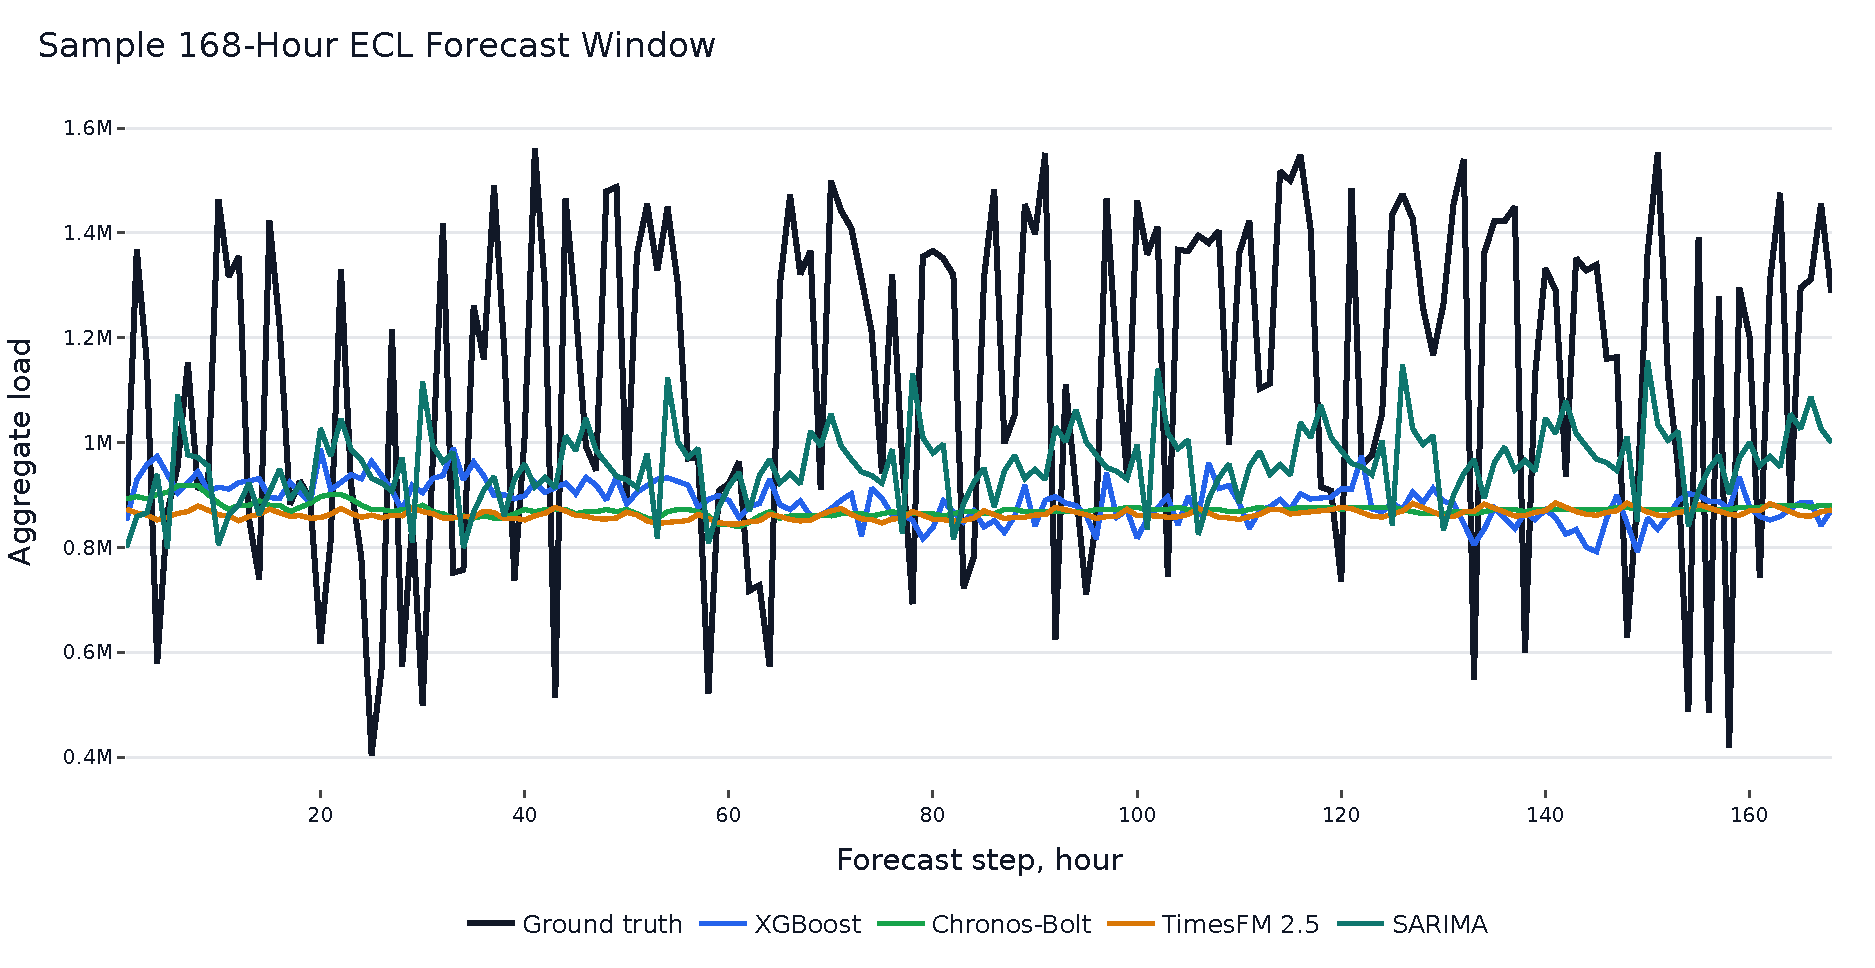
\includegraphics[width=\linewidth]{../figures/fig2_forecasts.pdf}
  \caption{Sample 168-hour ECL forecasts from representative models.}
  \label{fig:sample_forecasts}
\end{figure}

\begin{table}[t]
\centering
\caption{Accuracy on ECL test split.}
\label{tab:ecl_accuracy}
\resizebox{\linewidth}{!}{%
\begin{tabular}{llrrrr}
\toprule
Model & H & MAE & RMSE & sMAPE (\%) & wMAPE (\%) \\
\midrule
timesfm & 24 & 259345.28 & 307450.43 & 31.27 & 29.60 \\
chronos\_bolt\_small & 24 & 259546.11 & 311466.37 & 31.32 & 29.63 \\
xgboost & 24 & 259549.38 $\pm$ 13.62 & 306563.19 $\pm$ 18.53 & 31.33 $\pm$ 0.00 & 29.63 $\pm$ 0.00 \\
dlinear & 24 & 278309.93 $\pm$ 78.45 & 327075.05 $\pm$ 121.45 & 34.58 $\pm$ 0.01 & 32.94 $\pm$ 0.01 \\
patchtst & 24 & 279295.35 $\pm$ 274.56 & 328419.63 $\pm$ 622.11 & 34.68 $\pm$ 0.04 & 33.05 $\pm$ 0.03 \\
itransformer & 24 & 283321.32 $\pm$ 278.79 & 335735.87 $\pm$ 639.05 & 35.11 $\pm$ 0.03 & 33.53 $\pm$ 0.03 \\
seasonal\_naive & 24 & 338935.90 & 428088.82 & 39.98 & 38.69 \\
xgboost & 96 & 261792.58 $\pm$ 9.36 & 308906.88 $\pm$ 25.05 & 31.63 $\pm$ 0.00 & 29.94 $\pm$ 0.00 \\
chronos\_bolt\_small & 96 & 262601.94 & 314012.89 & 31.68 & 30.03 \\
timesfm & 96 & 262766.32 & 311382.39 & 31.65 & 30.05 \\
dlinear & 96 & 279227.54 $\pm$ 52.48 & 327146.57 $\pm$ 54.07 & 34.69 $\pm$ 0.01 & 33.07 $\pm$ 0.01 \\
itransformer & 96 & 279842.21 $\pm$ 148.37 & 327663.71 $\pm$ 205.90 & 34.75 $\pm$ 0.02 & 33.14 $\pm$ 0.02 \\
patchtst & 96 & 280109.77 $\pm$ 94.31 & 328333.77 $\pm$ 256.71 & 34.77 $\pm$ 0.02 & 33.17 $\pm$ 0.01 \\
seasonal\_naive & 96 & 340658.82 & 428618.32 & 40.13 & 38.96 \\
xgboost & 168 & 264220.96 $\pm$ 24.77 & 311145.57 $\pm$ 42.08 & 31.96 $\pm$ 0.00 & 30.30 $\pm$ 0.00 \\
chronos\_bolt\_small & 168 & 264268.27 & 315996.95 & 31.91 & 30.30 \\
timesfm & 168 & 265044.60 & 313676.28 & 31.95 & 30.39 \\
itransformer & 168 & 279476.02 $\pm$ 103.81 & 326253.85 $\pm$ 265.79 & 34.75 $\pm$ 0.01 & 33.15 $\pm$ 0.01 \\
dlinear & 168 & 280272.56 $\pm$ 47.26 & 328134.31 $\pm$ 38.84 & 34.84 $\pm$ 0.01 & 33.25 $\pm$ 0.01 \\
patchtst & 168 & 280876.20 $\pm$ 109.22 & 328943.70 $\pm$ 263.11 & 34.88 $\pm$ 0.01 & 33.32 $\pm$ 0.01 \\
seasonal\_naive & 168 & 343510.17 & 431537.72 & 40.48 & 39.39 \\
\bottomrule
\end{tabular}%
}
\end{table}

\begin{table}[t]
\centering
\caption{Accuracy on ETTH1 test split.}
\label{tab:etth1_accuracy}
\resizebox{\linewidth}{!}{%
\begin{tabular}{llrrrr}
\toprule
Model & H & MAE & RMSE & sMAPE (\%) & wMAPE (\%) \\
\midrule
chronos\_bolt\_small & 24 & 3.00 & 4.78 & 44.88 & 29.73 \\
patchtst & 24 & 3.04 $\pm$ 0.01 & 4.56 $\pm$ 0.01 & 47.47 $\pm$ 0.18 & 30.09 $\pm$ 0.11 \\
dlinear & 24 & 3.08 $\pm$ 0.00 & 4.63 $\pm$ 0.00 & 47.95 $\pm$ 0.10 & 30.53 $\pm$ 0.04 \\
timesfm & 24 & 3.16 & 4.88 & 48.33 & 31.25 \\
itransformer & 24 & 3.25 $\pm$ 0.02 & 4.77 $\pm$ 0.04 & 49.29 $\pm$ 0.09 & 32.17 $\pm$ 0.15 \\
seasonal\_naive & 24 & 3.31 & 5.44 & 46.07 & 32.78 \\
sarima & 24 & 3.45 & 4.92 & 52.92 & 34.15 \\
xgboost & 24 & 3.89 $\pm$ 0.01 & 5.40 $\pm$ 0.01 & 57.47 $\pm$ 0.08 & 38.50 $\pm$ 0.06 \\
dlinear & 96 & 3.55 $\pm$ 0.00 & 5.26 $\pm$ 0.01 & 54.11 $\pm$ 0.07 & 35.08 $\pm$ 0.02 \\
chronos\_bolt\_small & 96 & 3.57 & 5.61 & 51.08 & 35.30 \\
patchtst & 96 & 3.62 $\pm$ 0.03 & 5.27 $\pm$ 0.03 & 54.87 $\pm$ 0.36 & 35.79 $\pm$ 0.28 \\
timesfm & 96 & 3.67 & 5.61 & 54.27 & 36.24 \\
itransformer & 96 & 3.72 $\pm$ 0.01 & 5.43 $\pm$ 0.02 & 55.56 $\pm$ 0.24 & 36.81 $\pm$ 0.12 \\
sarima & 96 & 3.90 & 5.57 & 57.66 & 38.58 \\
seasonal\_naive & 96 & 3.92 & 6.41 & 51.70 & 38.80 \\
xgboost & 96 & 4.21 $\pm$ 0.01 & 5.86 $\pm$ 0.01 & 61.21 $\pm$ 0.04 & 41.63 $\pm$ 0.05 \\
dlinear & 168 & 3.70 $\pm$ 0.00 & 5.43 $\pm$ 0.01 & 56.49 $\pm$ 0.08 & 36.54 $\pm$ 0.02 \\
chronos\_bolt\_small & 168 & 3.77 & 5.85 & 53.36 & 37.20 \\
timesfm & 168 & 3.79 & 5.75 & 55.77 & 37.38 \\
itransformer & 168 & 3.91 $\pm$ 0.02 & 5.62 $\pm$ 0.03 & 57.87 $\pm$ 0.23 & 38.62 $\pm$ 0.23 \\
patchtst & 168 & 3.95 $\pm$ 0.07 & 5.62 $\pm$ 0.08 & 58.51 $\pm$ 0.74 & 38.96 $\pm$ 0.74 \\
sarima & 168 & 4.18 & 5.87 & 60.30 & 41.22 \\
seasonal\_naive & 168 & 4.18 & 6.70 & 54.20 & 41.26 \\
xgboost & 168 & 4.27 $\pm$ 0.01 & 5.98 $\pm$ 0.01 & 61.54 $\pm$ 0.04 & 42.15 $\pm$ 0.05 \\
\bottomrule
\end{tabular}%
}
\end{table}

\begin{table}[t]
\centering
\caption{Computational efficiency.}
\label{tab:efficiency}
\resizebox{\linewidth}{!}{%
\begin{tabular}{llrrrr}
\toprule
Model & Data/H & Train s & Infer ms & Params & GPU MB \\
\midrule
chronos\_bolt\_small & ecl/H24 & 0.000 & 15.6205 & 47718016 & 123.3 \\
dlinear & ecl/H24 & 11.795 & 55.8597 & 16176 & 26.3 \\
itransformer & ecl/H24 & 23.725 & 55.3372 & 311448 & 164.9 \\
patchtst & ecl/H24 & 43.077 & 55.7089 & 168280 & 608.6 \\
seasonal\_naive & ecl/H24 & 0.000 & 0.0041 & 0 & 0.0 \\
timesfm & ecl/H24 & 0.000 & 102.2329 & 200000000 & 895.6 \\
xgboost & ecl/H24 & 2.892 & 7.5029 & 57388 & 0.0 \\
chronos\_bolt\_small & ecl/H96 & 0.000 & 39.6397 & 47718016 & 345.8 \\
dlinear & ecl/H96 & 18.843 & 59.4035 & 64704 & 29.8 \\
itransformer & ecl/H96 & 31.380 & 66.2948 & 320736 & 165.0 \\
patchtst & ecl/H96 & 49.984 & 62.4020 & 361888 & 612.4 \\
seasonal\_naive & ecl/H96 & 0.000 & 0.0048 & 0 & 0.0 \\
timesfm & ecl/H96 & 0.000 & 91.9861 & 200000000 & 895.6 \\
xgboost & ecl/H96 & 10.485 & 25.0947 & 229423 & 0.0 \\
chronos\_bolt\_small & ecl/H168 & 0.000 & 45.2988 & 47718016 & 381.4 \\
dlinear & ecl/H168 & 25.996 & 64.1642 & 113232 & 32.7 \\
itransformer & ecl/H168 & 38.540 & 69.7238 & 330024 & 165.2 \\
patchtst & ecl/H168 & 56.942 & 75.2900 & 555496 & 617.3 \\
seasonal\_naive & ecl/H168 & 0.000 & 0.0058 & 0 & 0.0 \\
timesfm & ecl/H168 & 0.000 & 200.3501 & 200000000 & 896.4 \\
xgboost & ecl/H168 & 18.179 & 42.7073 & 401454 & 0.0 \\
chronos\_bolt\_small & etth1/H24 & 0.000 & 13.4838 & 47718016 & 123.3 \\
dlinear & etth1/H24 & 10.701 & 39.9808 & 16176 & 26.2 \\
itransformer & etth1/H24 & 20.171 & 39.1519 & 311448 & 164.8 \\
patchtst & etth1/H24 & 39.820 & 39.1007 & 168280 & 608.3 \\
seasonal\_naive & etth1/H24 & 0.000 & 0.0037 & 0 & 0.0 \\
timesfm & etth1/H24 & 0.000 & 98.1902 & 200000000 & 895.6 \\
xgboost & etth1/H24 & 2.340 & 6.1449 & 57417 & 0.0 \\
chronos\_bolt\_small & etth1/H96 & 0.000 & 36.2363 & 47718016 & 345.8 \\
dlinear & etth1/H96 & 9.899 & 39.2943 & 64704 & 29.8 \\
itransformer & etth1/H96 & 20.615 & 38.8574 & 320736 & 165.0 \\
patchtst & etth1/H96 & 38.598 & 39.9531 & 361888 & 612.6 \\
seasonal\_naive & etth1/H96 & 0.000 & 0.0052 & 0 & 0.0 \\
timesfm & etth1/H96 & 0.000 & 109.7588 & 200000000 & 895.6 \\
xgboost & etth1/H96 & 8.638 & 24.4694 & 229758 & 0.0 \\
chronos\_bolt\_small & etth1/H168 & 0.000 & 64.7316 & 47718016 & 381.4 \\
dlinear & etth1/H168 & 10.095 & 40.7118 & 113232 & 32.6 \\
itransformer & etth1/H168 & 21.127 & 44.3775 & 330024 & 165.1 \\
patchtst & etth1/H168 & 39.072 & 42.3925 & 555496 & 617.0 \\
seasonal\_naive & etth1/H168 & 0.000 & 0.0053 & 0 & 0.0 \\
timesfm & etth1/H168 & 0.000 & 208.5066 & 200000000 & 896.4 \\
xgboost & etth1/H168 & 14.775 & 42.6873 & 401899 & 0.0 \\
\bottomrule
\end{tabular}%
}
\end{table}


On ECL, the strongest group consists of XGBoost and the two foundation models. TimesFM has the lowest point-wise MAE at H=24, but the gap to XGBoost and Chronos-Bolt is below $0.1\%$, so the practical ranking among the three is essentially flat. XGBoost is then marginally best at H=96 and H=168, with Chronos-Bolt within roughly $0.3\%$ at all three horizons. The grid-tuned SARIMA tracks this top group within about $1.6$--$2.7\%$, comfortably ahead of the trained neural models. DLinear, PatchTST, and iTransformer improve substantially over SeasonalNaive but do not match the tree, foundation, or SARIMA models under the current training budget. The efficiency table (Table~\ref{tab:efficiency}) shows the practical trade-off under single-window latency measurement: SeasonalNaive and SARIMA have the lowest inference latencies, XGBoost remains faster than the neural and TimesFM models, Chronos-Bolt is competitive, and TimesFM is the slowest despite strong accuracy.

On ETTh1/HUFL, Chronos-Bolt is best at H=24, with PatchTST as the strongest trained model on the same horizon, while DLinear is best at H=96 and H=168. TimesFM is competitive but not the best on this benchmark. SARIMA is close to the best classical baseline and beats XGBoost across all three horizons---a notable role reversal versus ECL, where XGBoost dominates SARIMA. The results support the importance of including linear, transformer, foundation, and ARIMA-family baselines together: the best model class changes with dataset and horizon (Fig.~\ref{fig:heatmap}, Fig.~\ref{fig:horizon}).

\begin{table}[t]
\centering
\caption{Diebold--Mariano tests for top-2 models by MAE at seed 42.}
\label{tab:stat_tests}
\resizebox{\linewidth}{!}{%
\begin{tabular}{llrrr}
\toprule
Data/H & Comparison & Statistic & p-value & Sig. \\
\midrule
ecl/H24 & timesfm vs xgboost & 13.45 & <0.001 & True \\
ecl/H96 & xgboost vs chronos\_bolt\_small & -38.15 & <0.001 & True \\
ecl/H168 & xgboost vs chronos\_bolt\_small & -2.88 & 0.004 & True \\
etth1/H24 & chronos\_bolt\_small vs patchtst & -3.39 & <0.001 & True \\
etth1/H96 & dlinear vs chronos\_bolt\_small & -2.48 & 0.013 & True \\
etth1/H168 & dlinear vs chronos\_bolt\_small & -8.81 & <0.001 & True \\
\bottomrule
\end{tabular}%
}
\end{table}


The statistical tests confirm that the top comparisons are not only small numerical differences in flattened MAE. On ECL, the H=96 and H=168 results favor XGBoost over Chronos-Bolt; H=24 is nearly tied between TimesFM and XGBoost depending on whether one uses flattened point-wise MAE or per-window error aggregation, and although the Diebold--Mariano test rejects equal predictive accuracy, the absolute MAE difference is below $0.1\%$ and is likely operationally negligible. On ETTh1/HUFL, the tests support Chronos-Bolt at H=24 and DLinear at the two longer horizons. This strengthens the central observation that no single family dominates across datasets and horizons.

\begin{figure}[t]
  \centering
  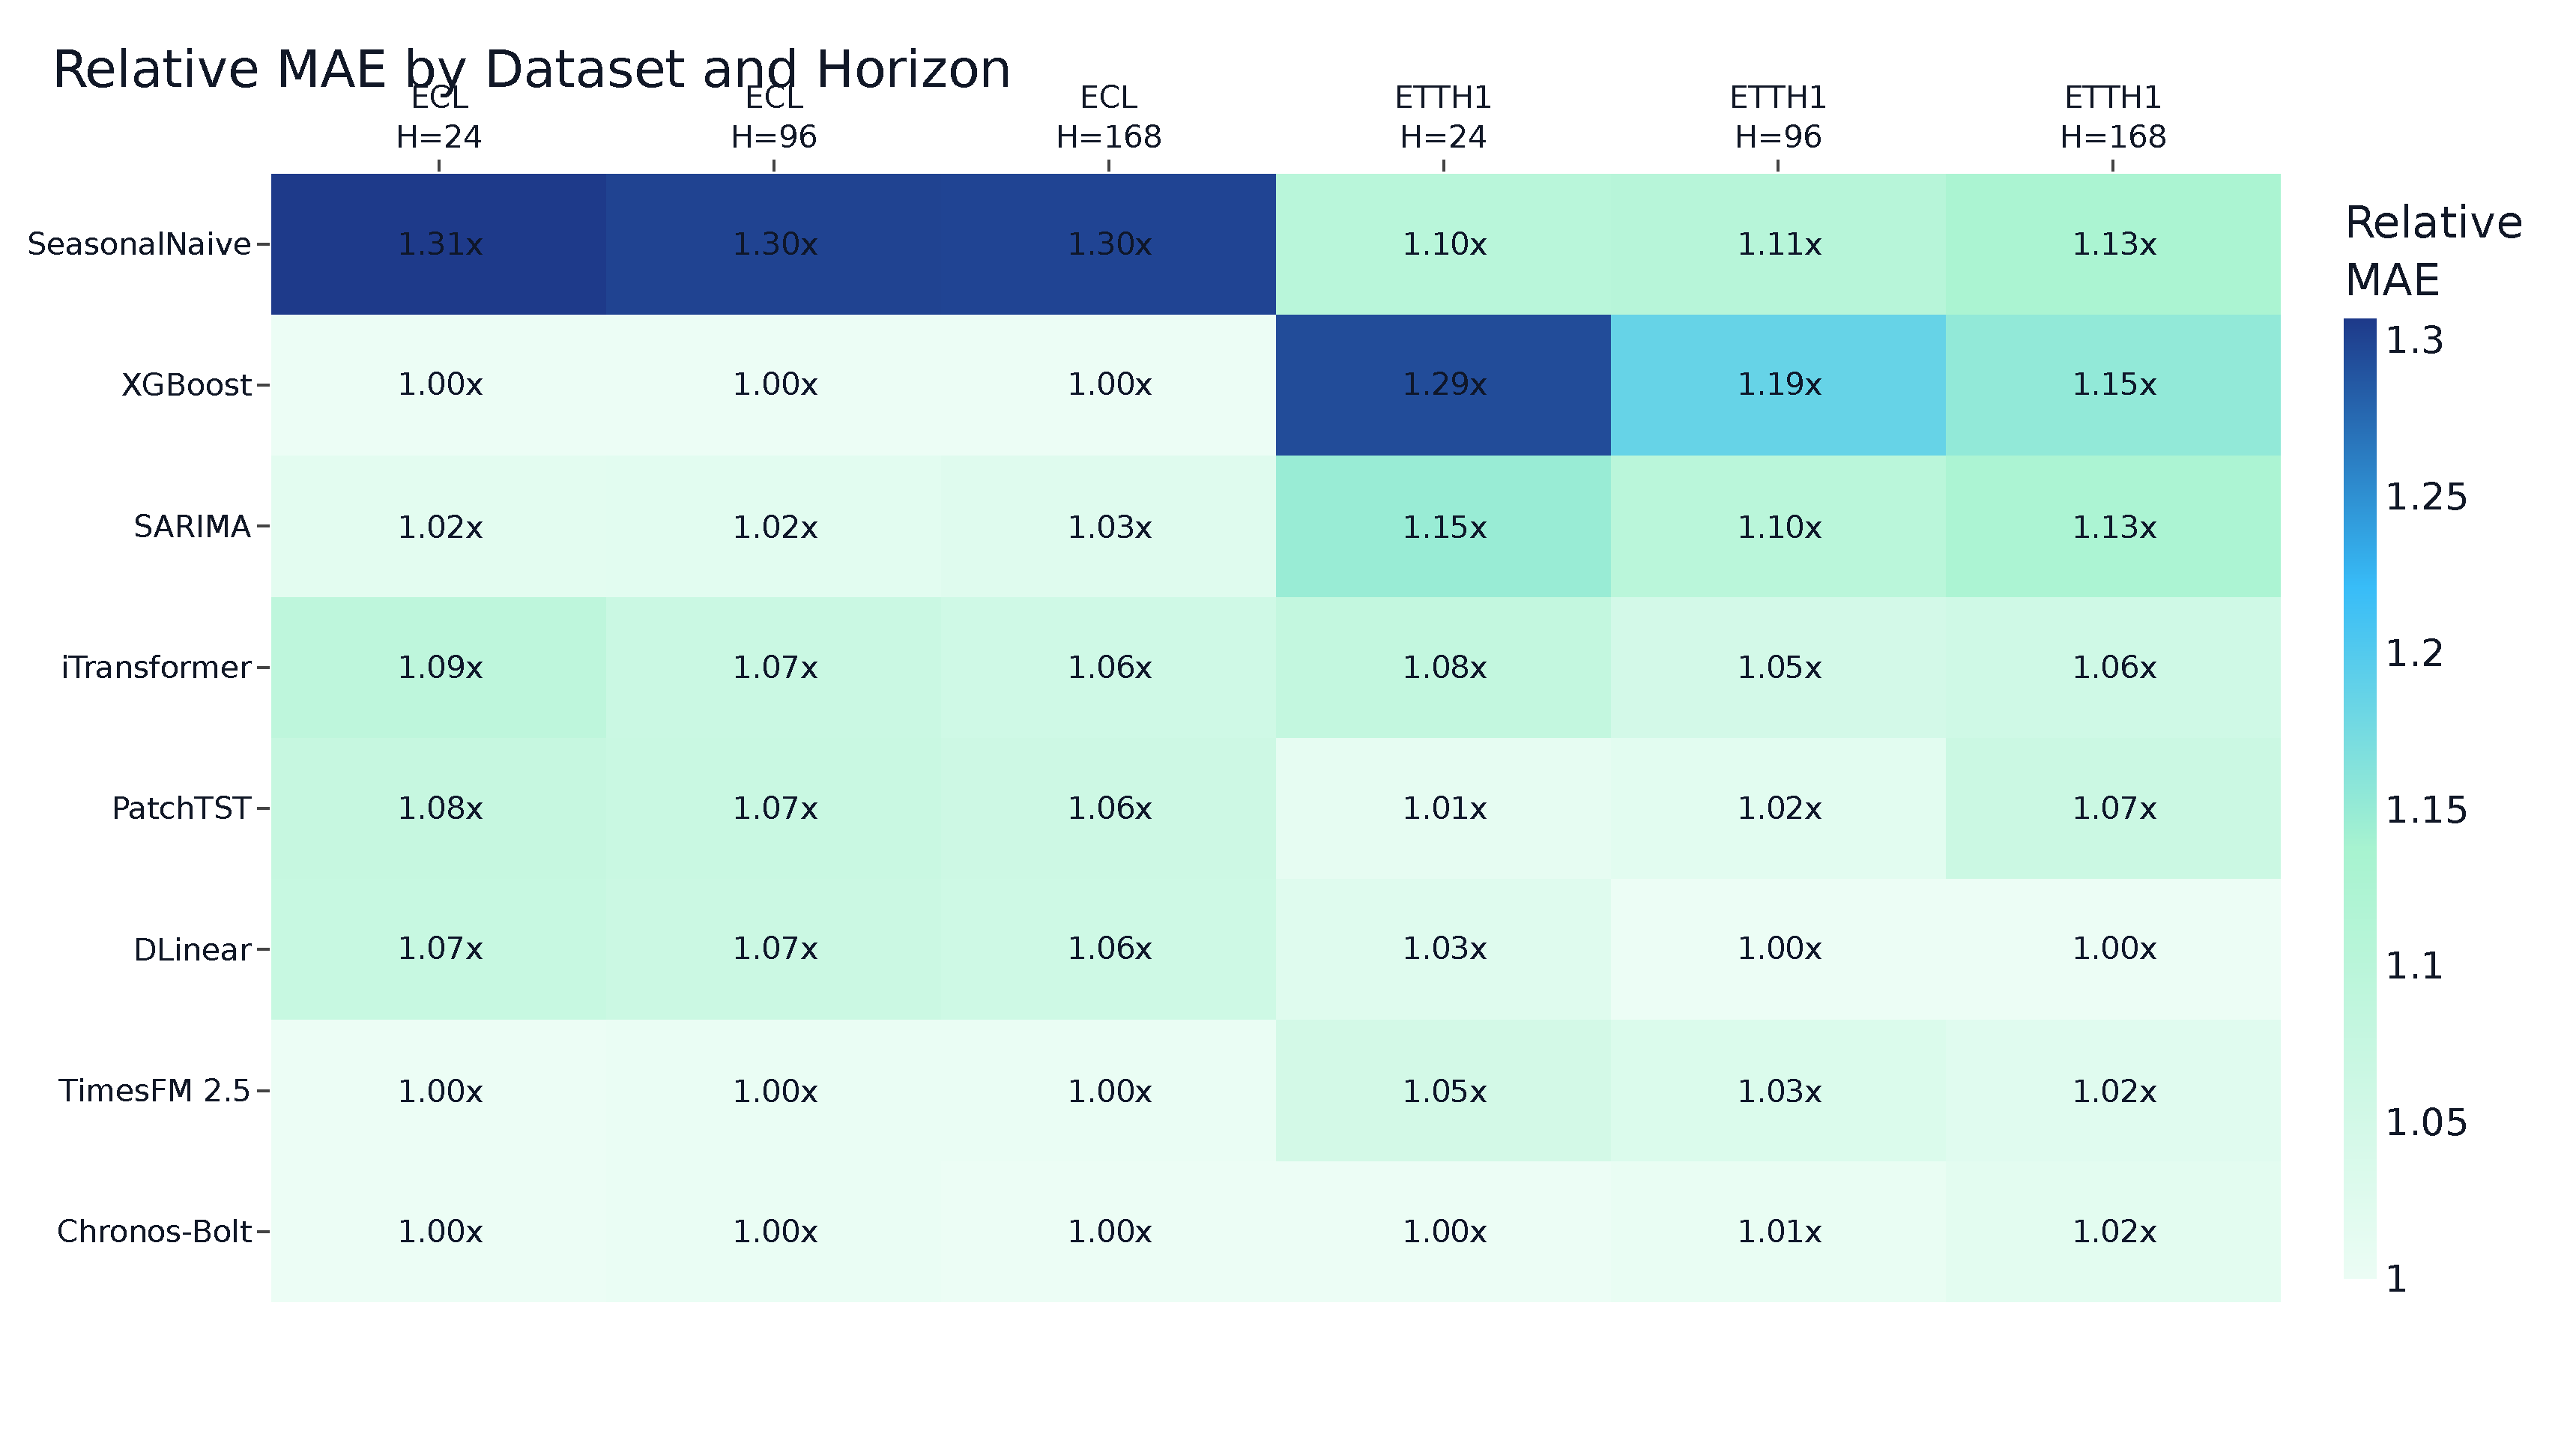
\includegraphics[width=\linewidth]{../figures/fig3_heatmap.pdf}
  \caption{MAE heatmap across executed datasets and horizons.}
  \label{fig:heatmap}
\end{figure}

\begin{figure}[t]
  \centering
  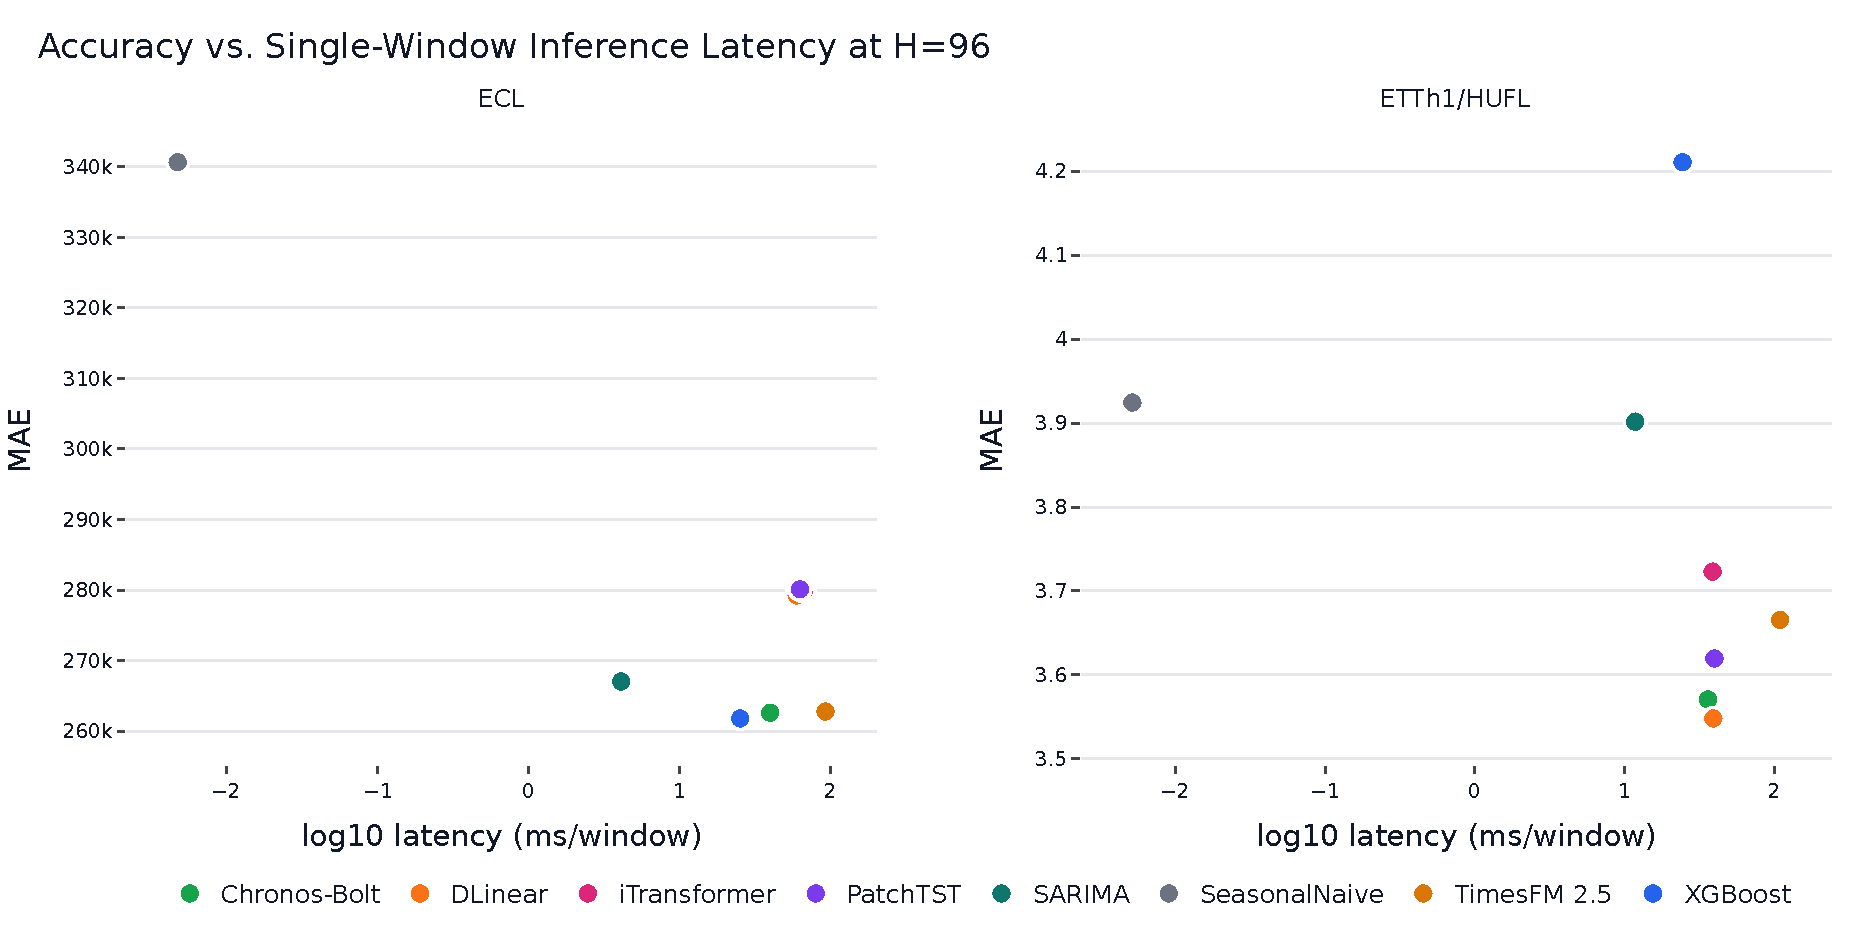
\includegraphics[width=\linewidth]{../figures/fig4_pareto.pdf}
  \caption{Accuracy--latency view at H=96.}
  \label{fig:pareto}
\end{figure}

\begin{figure}[t]
  \centering
  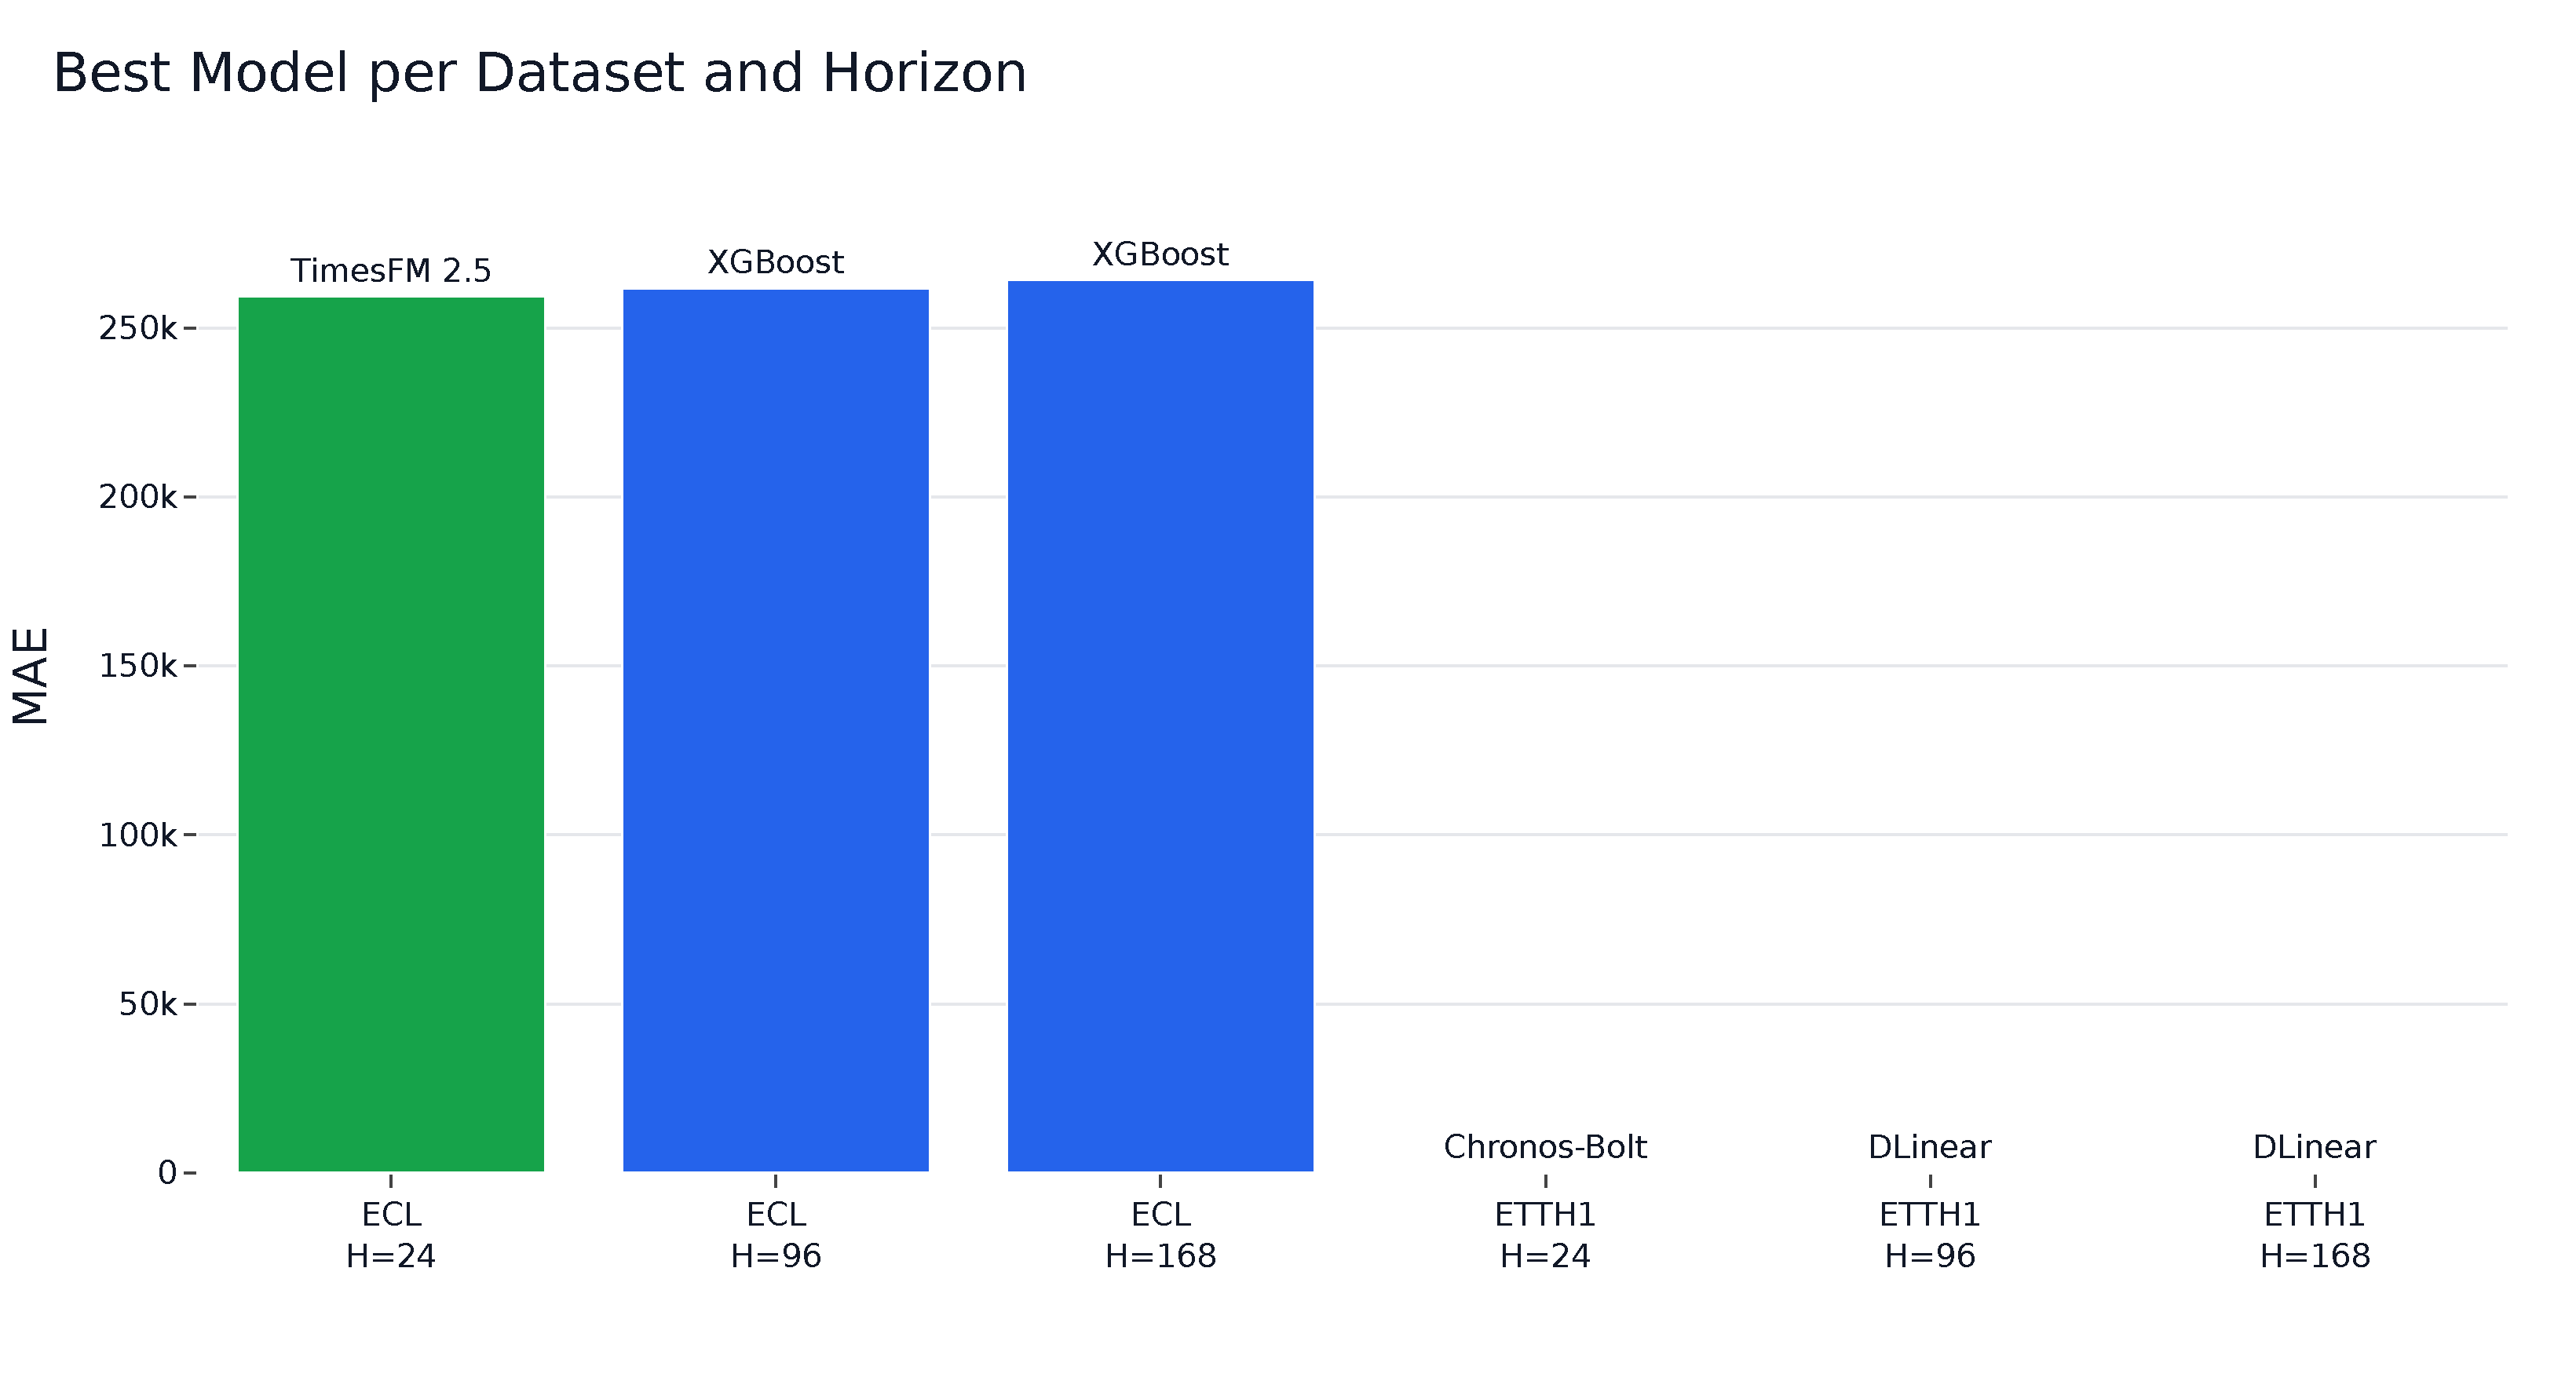
\includegraphics[width=\linewidth]{../figures/fig5_horizon.pdf}
  \caption{MAE by horizon for the executed model set.}
  \label{fig:horizon}
\end{figure}

\begin{figure}[t]
  \centering
  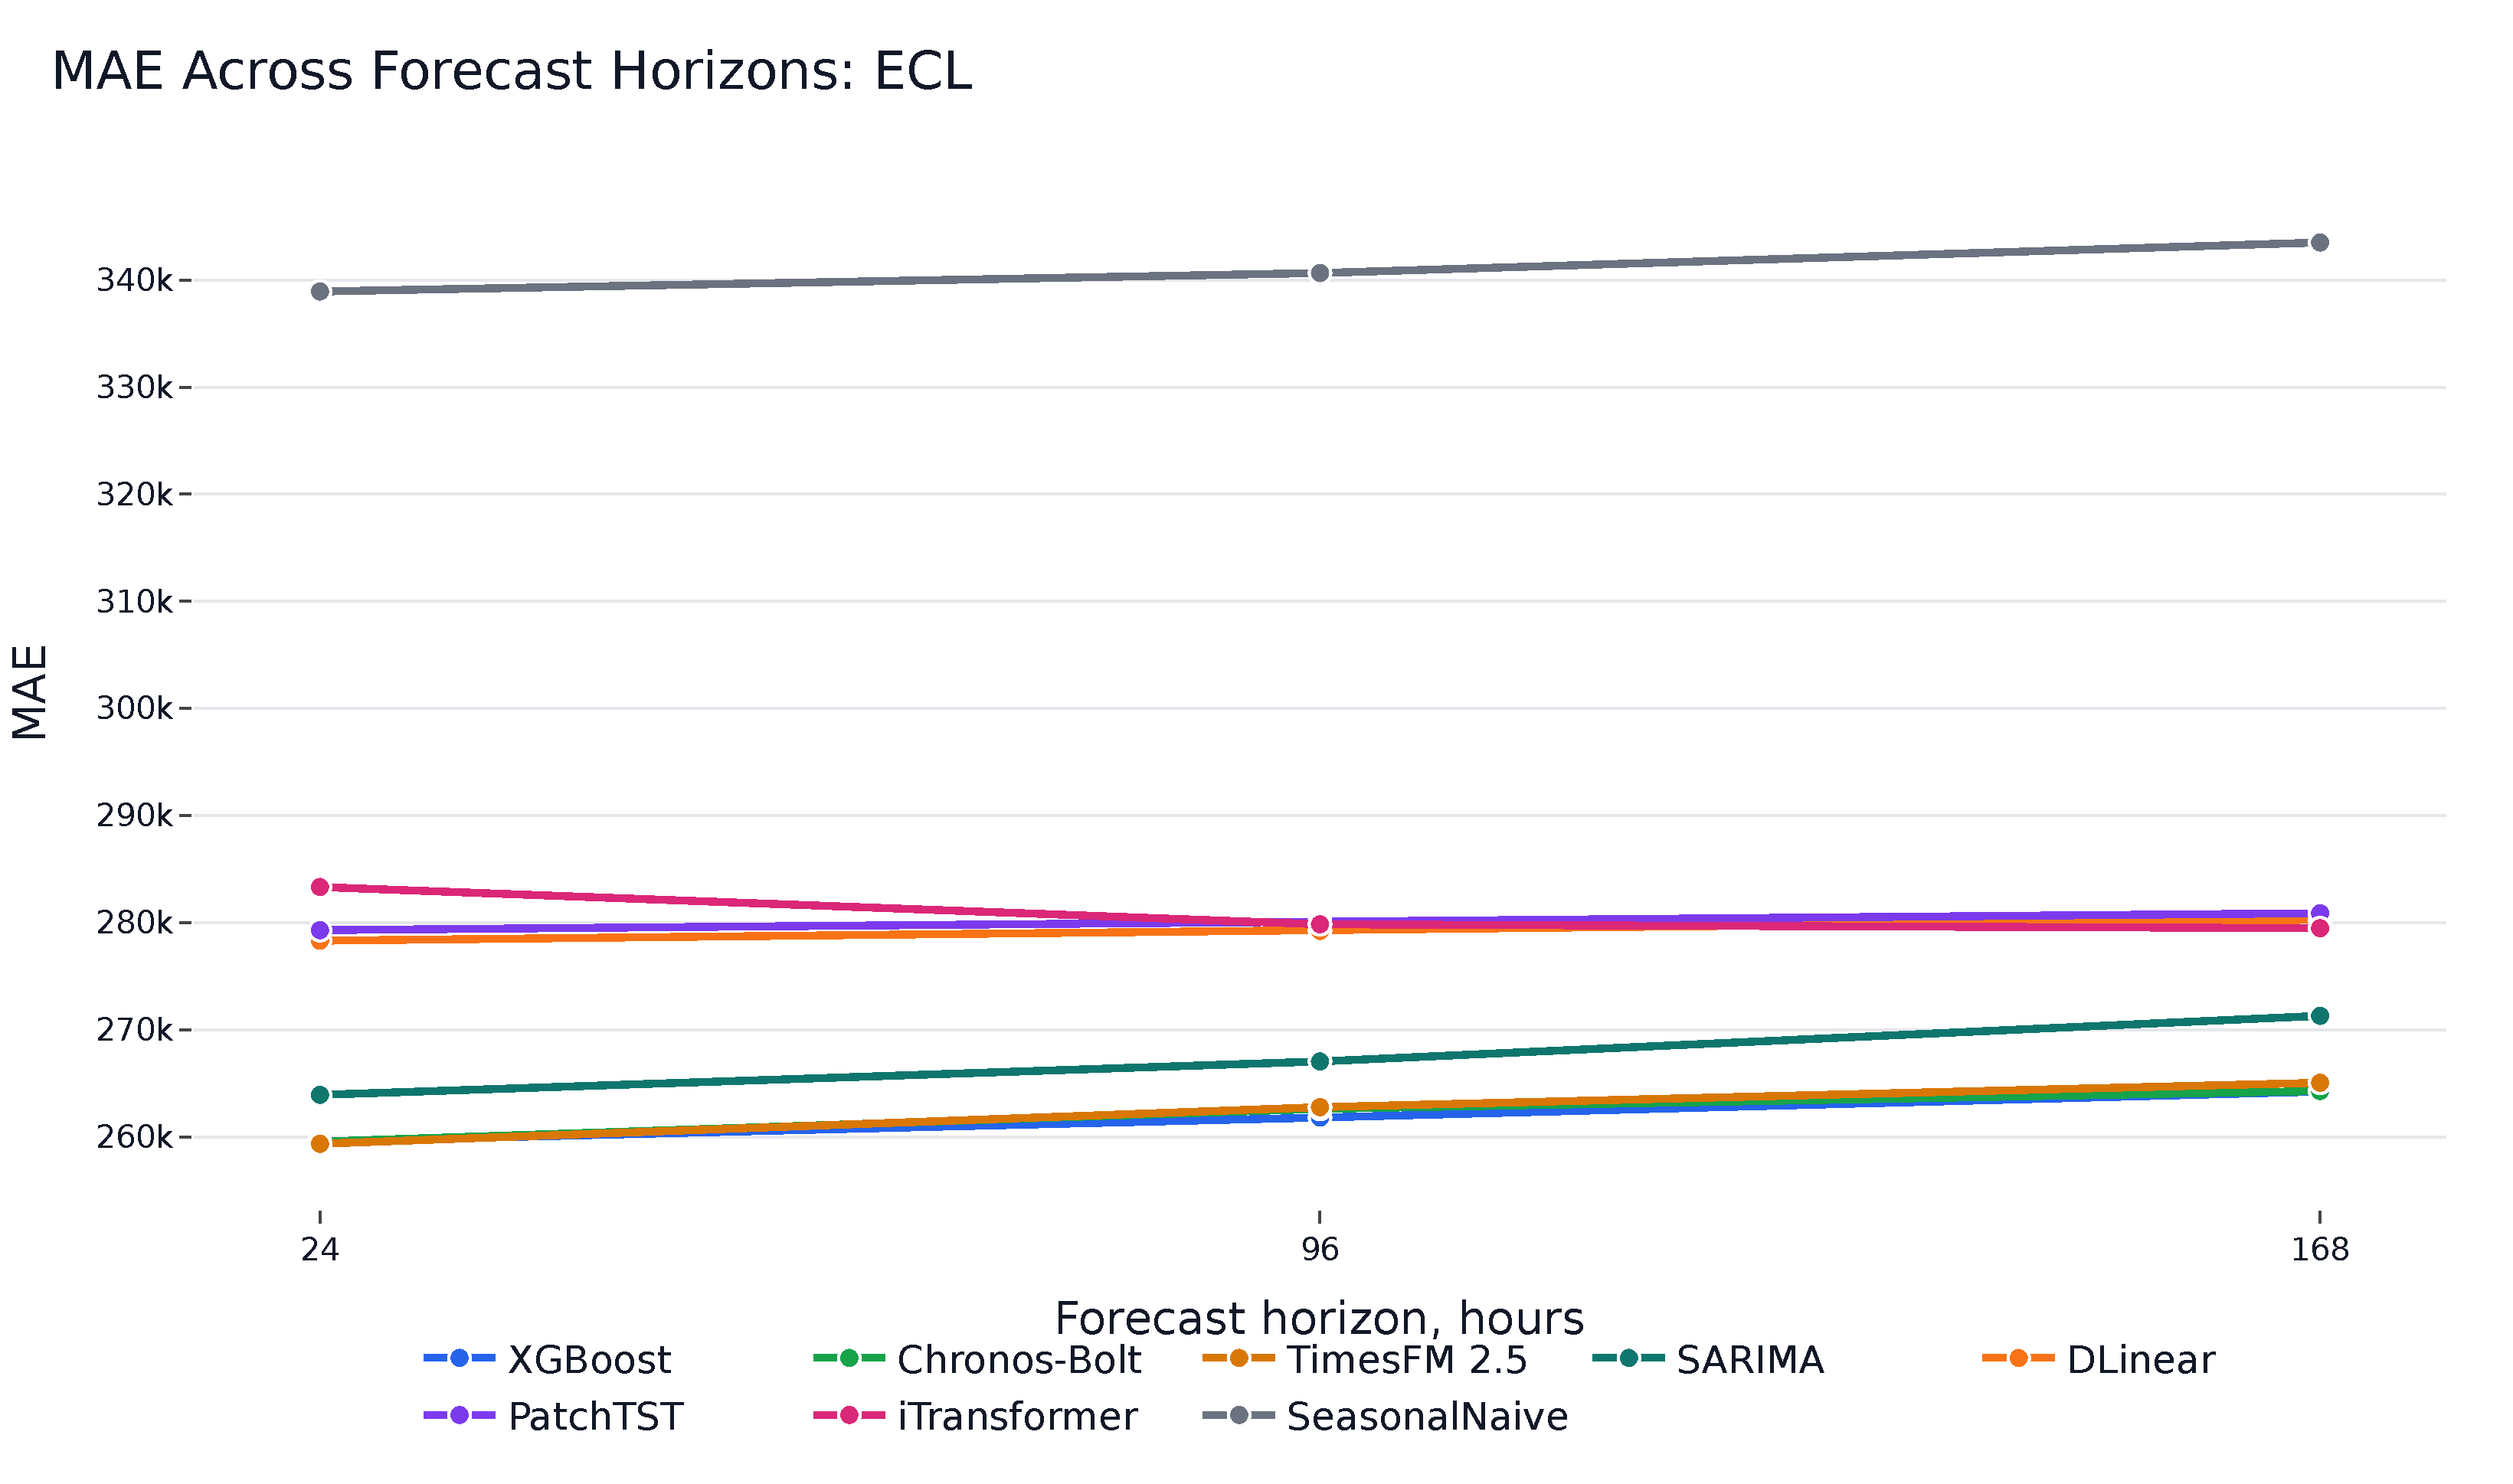
\includegraphics[width=\linewidth]{../figures/fig6_ecl_accuracy.pdf}
  \caption{MAE across forecast horizons on ECL.}
  \label{fig:ecl_accuracy}
\end{figure}

\begin{figure}[t]
  \centering
  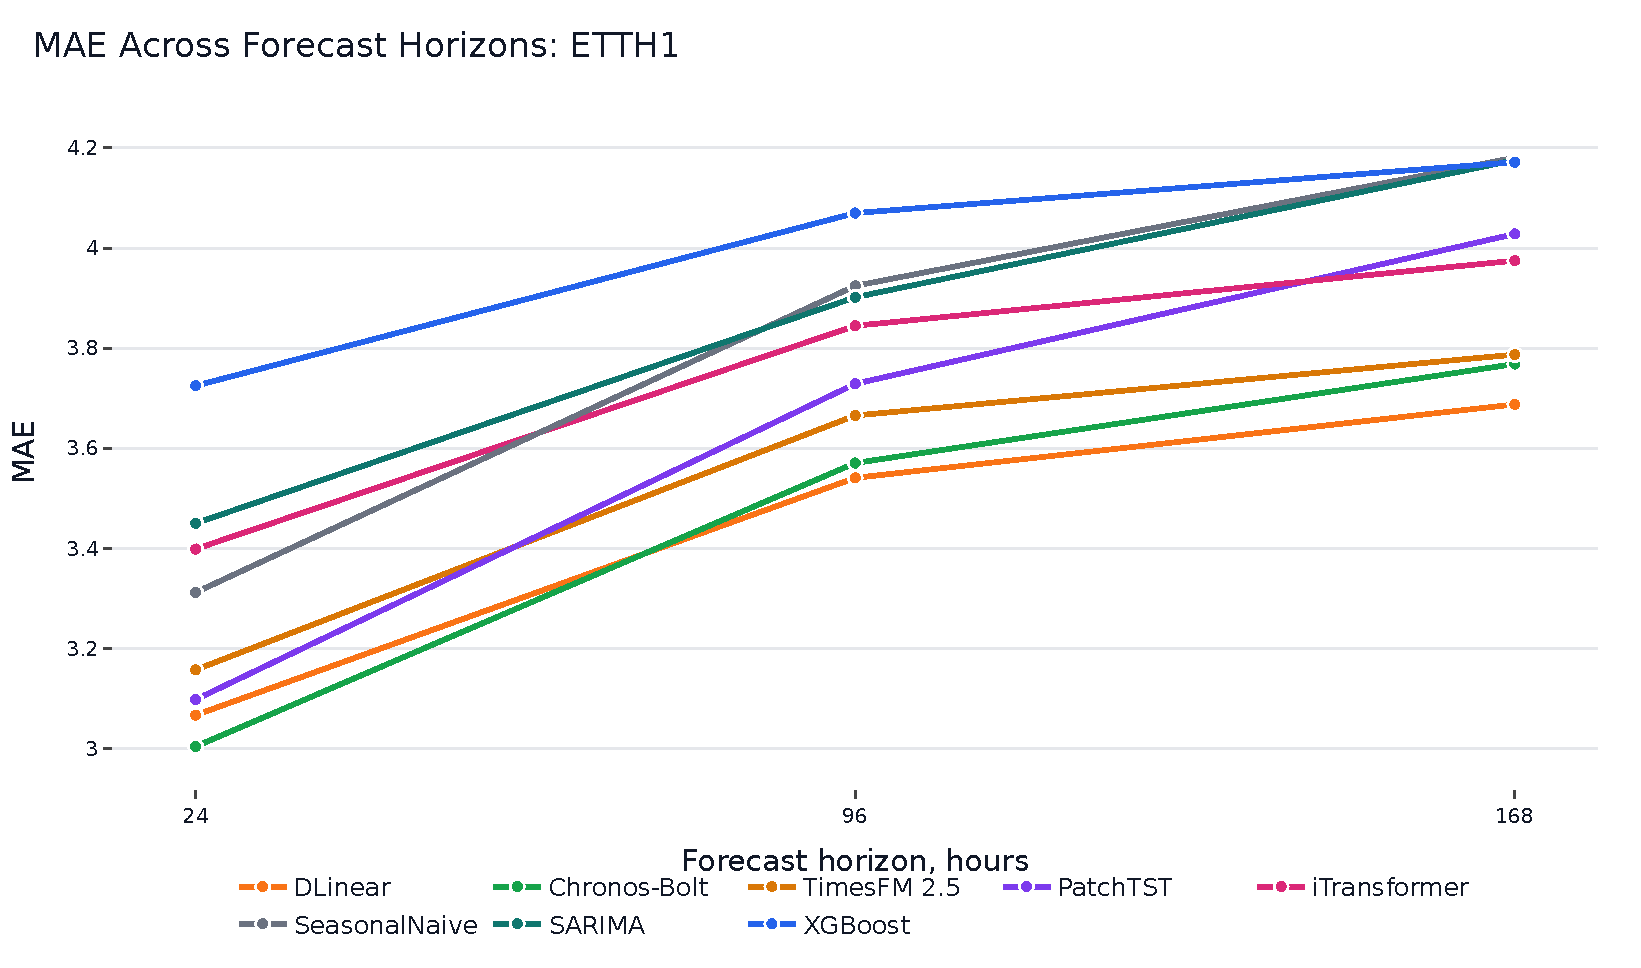
\includegraphics[width=\linewidth]{../figures/fig7_etth1_accuracy.pdf}
  \caption{MAE across forecast horizons on ETTh1/HUFL.}
  \label{fig:etth1_accuracy}
\end{figure}

The accuracy--latency view (Fig.~\ref{fig:pareto}) and the per-dataset MAE curves (Fig.~\ref{fig:ecl_accuracy}, Fig.~\ref{fig:etth1_accuracy}) make the operating regimes explicit and align with the table-level rankings.

\section{Discussion}
The results show that model choice is dataset-dependent. On aggregate ECL load, engineered lag features with XGBoost remain an extremely strong and inexpensive option, and a grid-tuned SARIMA is the next most accurate model, ahead of the trained neural architectures evaluated here. Foundation models are attractive when avoiding task-specific training is valuable: Chronos-Bolt is close to XGBoost on ECL and best at the shortest ETTh1/HUFL horizon. DLinear is the strongest trained neural model in this benchmark and dominates the longer ETTh1/HUFL horizons.

From a deployment perspective, the models occupy different operating regimes. XGBoost is the most attractive choice when a conventional supervised training pipeline is acceptable: it is accurate on ECL, has low single-window latency, and does not require GPU inference. SARIMA is a competitive low-cost backup with no learned features and millisecond inference. Chronos-Bolt is useful when task-specific training is undesirable, for example in cold-start industrial monitoring, rapid prototyping, or sites where historical data cannot be pooled for model training. TimesFM shows strong point accuracy at the shortest ECL horizon, but its latency is substantially higher in this implementation. DLinear is a good neural reference model because it is simple, compact, and strong on the longer ETTh1/HUFL horizons.

The transformer results should be read carefully. PatchTST and iTransformer are credible architectures, but this benchmark uses a compact target-only configuration and a fixed training budget. Their underperformance here does not imply that transformers are generally unsuitable for load forecasting; rather, it shows that they do not automatically beat simpler methods under constrained, reproducible settings. A production study should include a broader hyperparameter search, multivariate exogenous inputs, and possibly dataset-specific tuning.

The main limitations are public-benchmark pretraining-contamination risk for foundation models, limited hyperparameter search, target-only modeling, and the absence of private industrial deployment data. The SARIMA baseline is deliberately implemented as a practical fixed-order ARIMA-family reference: orders are selected on train by AICc and the parameters are reused for forecast windows, giving a fast and well-defined baseline rather than an expensive per-origin AutoARIMA search. Chronos-Bolt also emits a warning that prediction lengths above 64 are outside its recommended range; therefore, H=96 and H=168 Chronos results should be interpreted as practical stress tests rather than optimal use of that model.

The foundation-model results should also not be overinterpreted as guaranteed dataset-unseen zero-shot generalization. ECL and ETT are public benchmarks and may overlap with pretraining or evaluation corpora used during model development. The correct claim is therefore narrower: Chronos-Bolt and TimesFM were run without task-specific training in this repository. This remains practically relevant, but it is not the same as evaluating on a private unseen industrial dataset.

\section{Conclusion}
We built and executed a reproducible STLF benchmark pipeline on ECL and ETTh1/HUFL. On ECL, XGBoost, Chronos-Bolt, and TimesFM are statistically distinguishable but operationally near-tied within $0.4\%$, and a grid-tuned SARIMA is the closest follower; on ETTh1/HUFL, Chronos-Bolt wins H=24, PatchTST is the best trained model at H=24, and DLinear wins H=96 and H=168. These findings support a pragmatic recommendation: compare against strong simple baselines---including a properly tuned ARIMA-family model---first, use DLinear and PatchTST as neural references, and treat foundation models as valuable cold-start tools rather than universally dominant replacements for supervised forecasting.

\bibliographystyle{IEEEtran}
\bibliography{references}

\end{document}
